\maketitle
\setcounter{page}{1}
\tableofcontents
\newpage
\pagenumbering{arabic}
\section{Theorie}
Atomkerne zerfallen, wenn das Verhältnis zwischen Anzahl von Neutronen und Protonen
bestimmte Grenzen überschreitet. Eine wichtige Größe zum Zerfall von Atomen ist die
Halbwertszeit $T$. Diese bezeichnet den Zeitraum, in dem die Hälfte der instabilen Kerne
zerfallen ist. In diesem Versuch wird eine Methode diskutiert, die Halbwertszeit von Nukliden zu bestimmen,
deren $T$ in der Größenordnung Sekunden bis Stunden liegt. Da diese zu Beginn der Messung hergestellt
werden müssen, geschieht dies durch den Beschuss stabiler Kerne mit Neutronen, da diese die Coulomb-Barriere
nicht überwinden müssen. Im folgenden wird diese Kernreaktion betrachtet.

Sobald ein Neutron von einem Kern A aufgenommen wird,  entsteht ein neuer Kern A*, der Compound -
oder Zwischenkern genannt wird. Ihn unterscheidet von seinem Mutternuklid die kinetische und Bindungsenergie
des Neutrons. Diese Energie verteilt sich auf viele Nukleonen, die dadurch in höhere Energiezustände
gebracht werden. Deswegen ist es nicht möglich, dass der Kern das neue Nukleon oder ein anderes abstößt.
Aus diesem Grund geht der Kern nach der Emmission eines $\gamma$ - Quants wieder in seinen Grundzustand über:
\begin{equation*}
    \ce{^{m}_{z}A} + \ce{^{1}_{0} n} \rightarrow \ce{^{m + 1}_{z}A^*} \rightarrow \ce{^{m + 1}_{z}A} + \gamma
\end{equation*}
mit m als Massenzahl und z als Kernladungszahl. Der neue Kern $\ce{^{m + 1}_{z}A}$ ist nicht mehr stabil,
da er mehr Neutronen als ein stabiler Kern enthält. Er zerfällt nach längerer Zeit nach folgender Gleichung:
\begin{equation*}
    \ce{^{m + 1}_{z}A} \rightarrow \ce{^{m+1}_{z+1}C} + \symup{\beta}^- + E_{\symup{kin}} + \overline{\symup{\nu}}_{\symup{e}}
\end{equation*}
mit $\overline{\symup{\nu}}_{\symup{e}}$ als Antineutrino. Der Massendefekt in der obigen Gleichung wird
durch die kinetische Energie von Elektron und Antineutrino ausgeglichen.

Der Wirkungsquerschnitt $\sigma$ gibt die Wahrscheinlichkeit an, mit der ein Neutron von einem stabilen Kern
absorbiert wird. Er ist definiert durch
\begin{equation}
  \sigma = \frac{u}{nKd}
  \label{eqn:1}
\end{equation}
mit $u$ als Anzahl der Treffer, $n$ als Anzahl Neutronen pro Sekunde und $d$ als Dicke und $K$ als Atome pro $\symup{cm}^3$
einer \SI{1}{\centi\meter\squared} breiten Folie. Der Wirkungsquerschnitt ist stark geschwindigkeitsanhängig.
Wenn die Geschwindigkeit des Neutrons hoch genug ist, dass die De-Broglie Wellenlänge klein gegen den Radius
des Kerns ist, kann geometrische Optik angewendet werden und es müssen keine Interferenzeffekte betrachtet werden.
Damit Resonanzabsorption auftritt muss die Energie des Neutrons der Differenz zweier Energieniveaus von A* entsprechen.
Aus einer Formel von Breit und Wigner folgt somit die Relation
\begin{equation*}
  \sigma \propto \frac{1}{v} \, .
\end{equation*}
Daraus wird bestätigt, dass bei kleinen Geschwindigkeiten die Wahrscheinlichkeit steigt, dass
das Neutron vom Kern aufgenommen wird.\\
\\
Da Neutronen als freie Teilchen instabil sind, müssen sie vor dem Versuch erzeugt werden. Dabei läuft
folgende Reaktion ab:
\begin{equation*}
  \ce{^{9}_{4}Be} + \ce{^{4}_{2}He} \rightarrow \ce{^{12}_{6}C} + \ce{^{1}_{0}\symup{n}}
\end{equation*}
Die $\alpha$-Teilchen stammen aus dem Zerfall von $\ce{^{226}Ra}$. Die Neutronen werden noch abgebremst,
da aufgrund obiger Überlegungen niederenergetische Neutronen am besten geeignet sind. Zu diesem Zweck
werden die Neutronen auf dicke Materieschichten mit leichten Atomkernen geschossen, damit sie wegen
elastischen Stößen Energie abgeben. Aus dem Gesetz zum elatischen Stoß folgt, dass die Energieübertragung
maximiert wird, falls die Massen der Stoßpartner gleich sind. Dafür bietet sich Wasserstoff an.
Der Aufbau zur Erzeugung der niederenergetischen Elektronen ist in Abbildung \ref{fig:2} abgebildet.
\begin{figure}
  \centering
  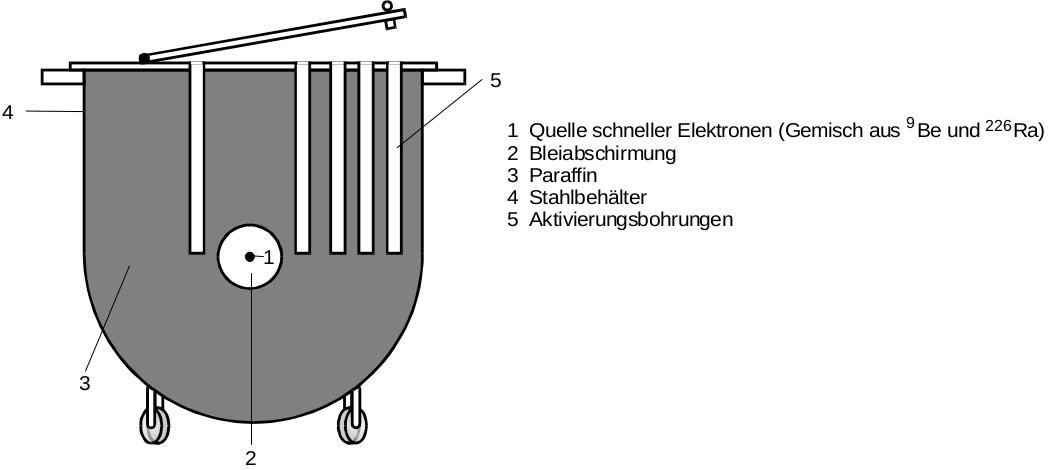
\includegraphics[scale=0.4]{quelle.png}
  \caption{Quelle zur Erzeugung von niederenergetischen Neutronen \cite{anleitung}.}
  \label{fig:2}
\end{figure}
Die Neutronen, die diese Apparatur verlassen, haben eine Energie von \SI{0.025}{\electronvolt}. Diese entspricht
einer Temperatur von \SI{290}{\kelvin}. Daraus folgt eine mittlere Neutronengeschwindigkeit von \SI{2.2}{\kilo\meter\per\second}.
Solche Neutronen werden als thermische Neutronen bezeichnet. \\
\\
In diesem Versuch werden folgende Zerfälle untersucht:
\begin{align}
  \ce{^{115}_{49}In} \, +& \, \symup n \rightarrow   \ce{^{116}_{49}In} \rightarrow  \ce{^{116}_{50}Sn} + \symup{\beta}^- + \overline{\symup{\nu}}_{\symup{e}} \\
  \ce{^{107}_{47}Ag} \, +& \, \symup n \rightarrow   \ce{^{108}_{47}Ag} \rightarrow  \ce{^{108}_{50}Cd} + \symup{\beta}^- + \overline{\symup{\nu}}_{\symup{e}} \label{eqn:2}\\
  \ce{^{109}_{47}Ag} \, +& \, \symup n \rightarrow   \ce{^{110}_{47}Ag} \rightarrow  \ce{^{110}_{48}Cd} + \symup{\beta}^- + \overline{\symup{\nu}}_{\symup{e}} \label{eqn:3}
\end{align}
Dabei ist jedoch für Silber eine Besonderheit zu beachten: Silber liegt in der Natur zu 52,3 \% als $\ce{^{107}Ag}$
und zu 48,7 \% als $\ce{^{109}Ag}$. Die Zerfälle \eqref{eqn:2} und \eqref{eqn:3} laufen gleichzeitig ab und
die Gesamtaktivität besteht aus der Addition der beiden Einzelaktivitäten. Da $\ce{^{110}Ag}$ aber sehr kurzlebig
ist, kommt nach einiger Zeit $t^*$ sämtliche Aktivität nur noch von $\ce{^{108}Ag}$ (siehe Abbildung \ref{fig:3}). Über diese Relation und das
Zerfallsgesetz
\begin{equation}
  N(t) = N_0 \, e^{-\mu t}
  \label{eqn:4}
\end{equation} mit $\mu$ als Zerfallskonstante und $N_0 = N(0)$ lassen sich die beiden Halbwertszeiten getrennt voneinander bestimmen.
\begin{figure}
  \centering
  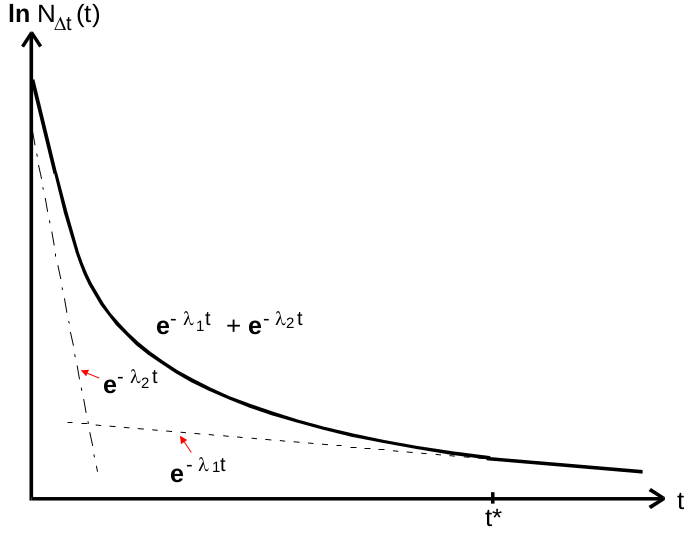
\includegraphics[scale=0.4]{silber.png}
  \caption{Zerfallsdiagramm eines Materials, dass zwei unterschiedlich langelebige Isotope besitzt \cite{anleitung}.}
  \label{fig:3}
\end{figure}

Aus \eqref{eqn:4} folgt für die Halbwertszeit
\begin{equation}
  T = \symup{ln}(2) / \mu \, .
  \label{eqn:5}
\end{equation}
Da die Bestimmung von $N(t)$ nicht ohne weiteres möglich ist, wird eine neue Größe
$N_{\symup{\Delta}t}(t)$ eingeführt. Diese wird definiert als
\begin{equation}
  N_{\symup{\Delta}t}(t) = N(t) - N(t + \symup{\Delta}t)
  \label{eqn:6}
\end{equation}
mit $\symup{\Delta}t$ als beliebigem Zeitintervall. Aus \eqref{eqn:4} folgt mit der Definition
\eqref{eqn:6}
\begin{equation}
  \symup{ln}[N_{\symup{\Delta}t}(t)] = \symup{ln}\left[N_0 (1 - \symup{e}^{- \mu \symup{\Delta}t})\right] - \mu t \, .
  \label{eqn:7}
\end{equation}
Aus \eqref{eqn:7} lässt sich mittels linearer Ausgleichsrechnung $\mu$ und damit aus \eqref{eqn:5}
$T$ bestimmen. Das Zeitintervall $\symup{\Delta}t$ ist dabei von Material zu Material unterschiedlich
und wird angegeben.

\section{Durchführung}
\subsection{Versuchsaufbau}
Der Versuchsaufbau ist in \ref{fig:4} zu sehen. Mit dem Geiger-Müller-Zählrohr werden
die Zerfälle nachgewiesen, wobei die Bleiummantelung den Einfluss der Umgebungsstrahlung
und die Strahlung außerhalb des Versuchsaufbaus
minimieren soll. Das Gerät zum Anzeigen der Zerfälle hat dabei zwei Speicherplätze,
die laufend überschrieben werden. Das Zeitintervall, in dem gemessen werden soll,
lässt sich am Gerät einstellen.
\begin{figure}
  \centering
  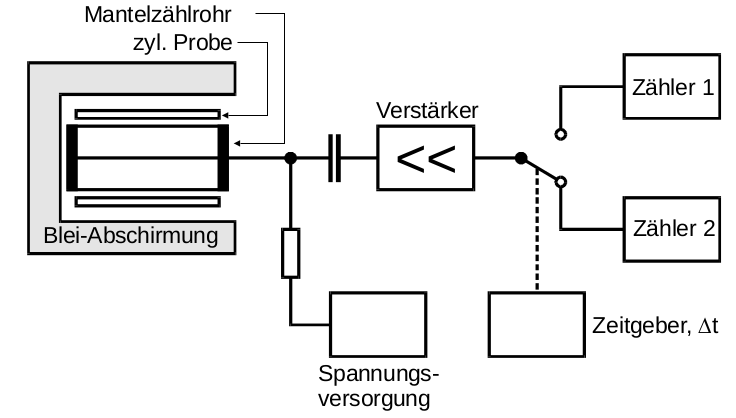
\includegraphics[scale=0.4]{aufbau.png}
  \caption{Schematischer Versuchsaufbau. \cite{anleitung}}
  \label{fig:4}
\end{figure}

\subsection{Versuchsdurchführung}
Zuerst wurde \SI{900}{\second} lang der Nulleffekt gemessen. Danach werden für Indium 15 Messwerte
mit einem Zeitintervall $\symup{\Delta}t = \SI{4}{\minute}$ und für Silber 53 Messwerte mit einem
Zeitintervall $\symup{\Delta}t = \SI{8}{\second}$ bestimmt.

\section{Auswertung}
\subsection{Behandlung der Messwerte}
Die gemessenen Vorgänge unterliegen einer Poission-Verteilung, der Fehler eines
Messwertes $x_i$ ist somit durch $\sqrt{x_i}$ gegeben. Die dargestellten Ausgleichsrechnungen
wurden durch die Funktion \textsc{curve-fit} aus dem \textsc{python}-Paket \textsc{scipy.optimise}
durchgeführt. Finden fehlerbehaftete Größen
in Formeln Anwendung, wird der resultierende Fehler in \textsc{uncertainties} bestimmt.
\subsection{Nullmessung}
Es werden innerhalb von \SI{900}{\second} \num{164} Ausschläge am Geiger-Müller-Zählrohr
gemessen. Dies entspricht einem Wert von $N_\symup{null} = \SI[per-mode=reciprocal]{0.18}{\per\second}$.
Dieser Wert ist zwar gering, aber gerade bei längeren Messintervallen statistisch
signifikant, sodass er von den Messwerten abgezogen werden muss.
\subsection{Messung von Indium}
\begin{figure}[h]
  \centering
    \begin{subfigure}{0.74\textwidth}
    \centering
      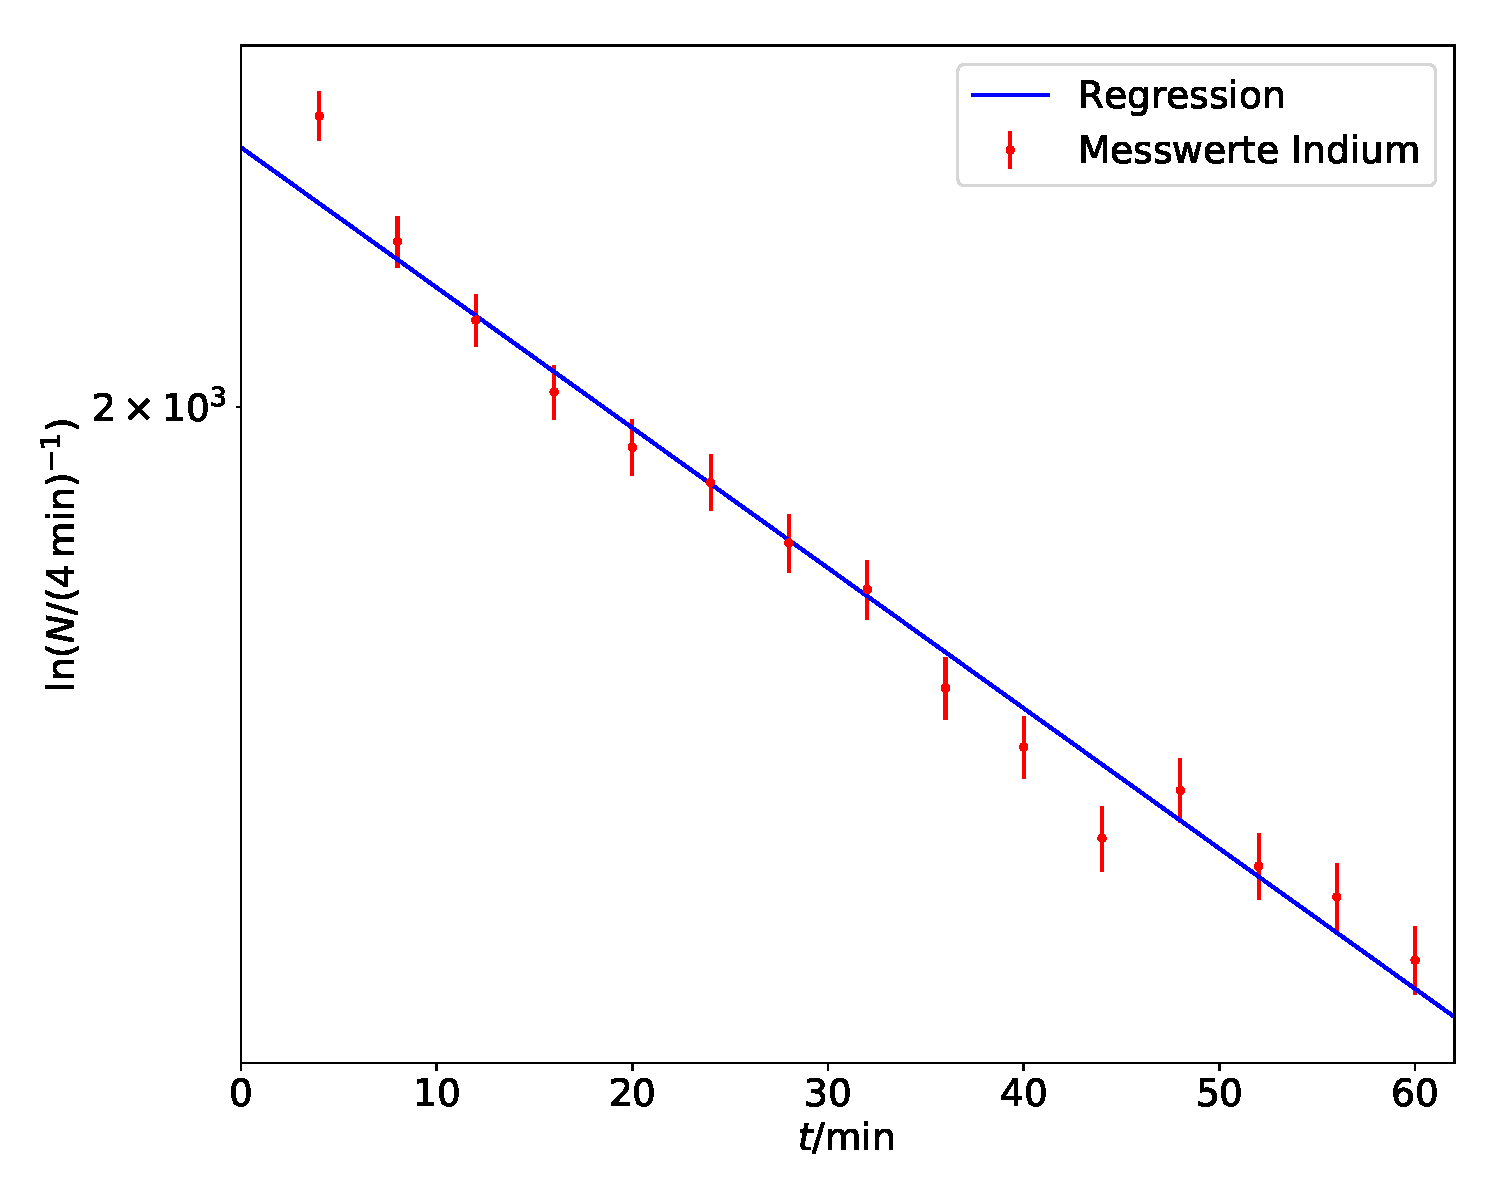
\includegraphics[width=\textwidth]{Indium.pdf}
      \caption{Grafische Darstellung der Messwerte mit Regression.}
      \label{fig:5}
    \end{subfigure}
    \begin{subtable}{0.25\textwidth}
      \centering
      \begin{tabular}{c c c}
        \toprule
        $t$ / \si{\minute} & $N$ & $\sigma_\symup{N}$ \\
        \midrule
        4 & 2540 & 50 \\
        8 & 2291 & 48 \\
        12 & 2148 & 46 \\
        16 & 2025 & 45 \\
        20 & 1935 & 44 \\
        24 & 1880 & 43 \\
        28 & 1789 & 42 \\
        32 & 1722 & 42 \\
        36 & 1588 & 40 \\
        40 & 1513 & 39 \\
        44 & 1404 & 37 \\
        48 & 1460 & 38 \\
        52 & 1372 & 37 \\
        56 & 1338 & 37 \\
        60 & 1270 & 36 \\
        \bottomrule
      \end{tabular}
      \caption{Messwerte.}
      \label{tab:1}
    \end{subtable}
    \caption{In Tabelle \subref{tab:1} sind die für das Isotop
    $\ce{^{116}In}$ gemessenen Werte mit Fehler $\sigma_\symup{N} = \sqrt{N}$ eingetragen. Diese Werte sind
    vom Nulleffekt bereinigt. In Grafik \subref{fig:5} findet sich die
    halblogarithmische Darstellung der vom Nulleffekt bereinigten Messwerte mit
    einer linearen Regression.}
  \end{figure}
  Die Messwerte finden sich in Tabelle \ref{tab:1}. Die Werte verhalten sich nach \eqref{eqn:4}.
Die Regression wird nach \eqref{eqn:7} ausgeführt. Mit \eqref{eqn:5} ergeben sich also folgende Konstanten:
  \begin{align*}
    \mu_\symup{In} =& \, \SI[per-mode=reciprocal]{1.92(8)e-4}{\per\second} \\
    N_{0\symup{, In}} =& \, \num[per-mode=reciprocal]{2.48(5)e3}\\
    T_{\symup{In}} =& \, \SI{60.2(25)}{\minute}.
  \end{align*}
Die Messwerte mit Fehler sowie die berechnete Regression finden sich in Abbildung \ref{fig:5}.
\subsection{Messung von Silber}
\begin{table}
  \centering
  \begin{tabular}{c c c | c c c | c c c | c c c}
    \toprule
    $t$ / \SI{8}{\second} & $N$ & $\sigma_\symup{N} $ & $t$ / \SI{8}{\second} &
     $N$ & $\sigma_\symup{N} $ & $t$ / \SI{8}{\second} & $N$ & $\sigma_\symup{N} $
     & $t$ / \SI{8}{\second} & $N$ & $\sigma_\symup{N} $\\
    \midrule
    8 & 145 & 12 & 112 & 23 & 5 & 216 & 8 & 3 & 320 & 9 & 3 \\
    16 & 119 & 11 & 120 & 20 & 4 & 224 & 5 & 2 & 328 & 9 & 3 \\
    24 & 85 & 9 & 128 & 17 & 4 & 232 & 5 & 2 & 336 & 5 & 2 \\
    32 & 86 & 9 & 136 & 21 & 5 & 240 & 10 & 3 & 344 & 5 & 2 \\
    40 & 59 & 8 & 144 & 15 & 4 & 248 & 9 & 3 & 352 & 2  & 1 \\
    48 & 57 & 8 & 152 & 21 & 5 & 256 & 2 & 1 & 360 & 3  & 2 \\
    56 & 42 & 6 & 160 & 16 & 4 & 264 & 3 & 2 & 368 & 14 & 4 \\
    64 & 50 & 7 & 168 & 14 & 4 & 272 & 9 & 3 & 376 & 4  & 2 \\
    72 & 33 & 6 & 176 & 4  & 2 & 280 & 8 & 3 & 384 & 4  & 2 \\
    80 & 23 & 5 & 184 & 10 & 3 & 288 & 4 & 2 & 392 & 8  & 3 \\
    88 & 23 & 5 & 192 & 11 & 3 & 296 & 8 & 3 & 408 & 4  & 2 \\
    96 & 25 & 5 & 200 & 12 & 3 & 304 & 9 & 3 & 416 & 8  & 3 \\
    104 & 22 & 5 & 208 & 8 & 3 & 312 & 5 & 2 & 424 & 4 & 2 \\
    \bottomrule
  \end{tabular}
  \caption{Messwerte der Messung an Silberisotopen mit Fehler $\sigma_\symup{N} = \sqrt{N}$.}
  \label{tab:2}
\end{table}
\begin{figure}
\centering
  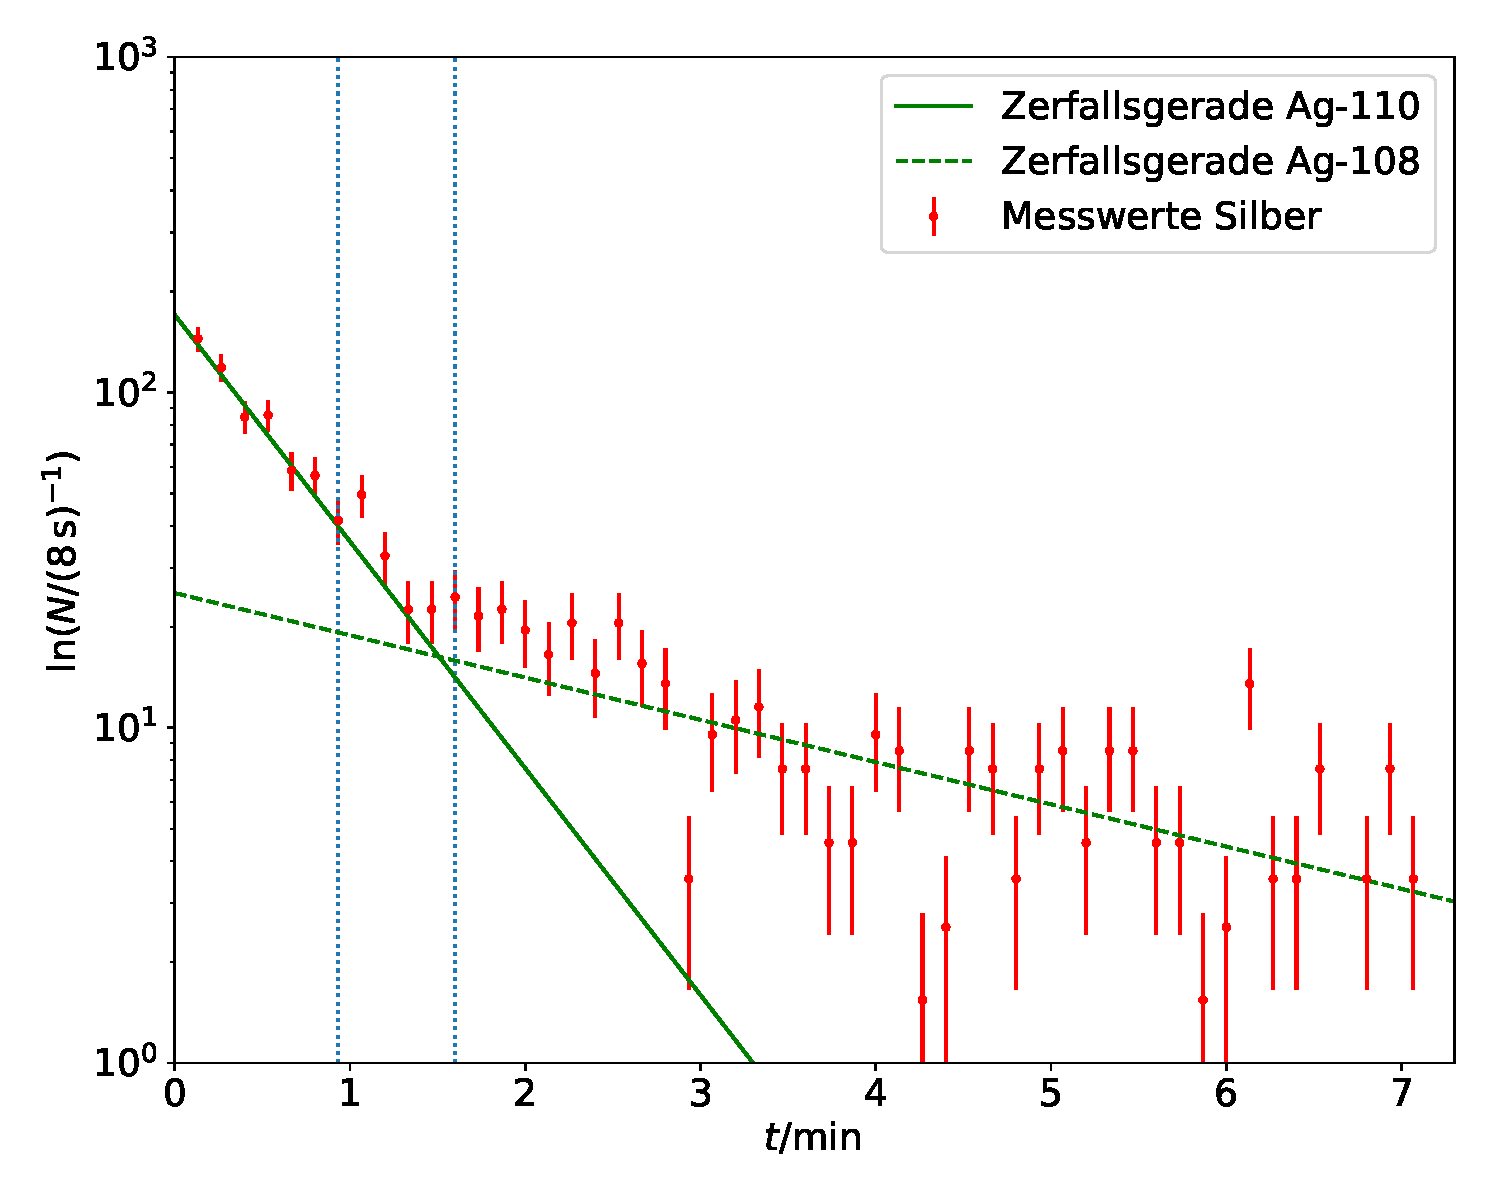
\includegraphics[width=\textwidth]{Silber.pdf}
  \caption{Diagramm der vom Nulleffekt bereinigten Messwerte.
   Ebenfalls eingetragen sind die Zerfallsgeraden
  der Isotope $\ce{^{108}Ag}$ und $\ce{^{110}Ag}$.}
  \label{fig:6}
\end{figure}
Die Messwerte finden sich in Tabelle \ref{tab:2}. Die halblogarithmische Darstellung
der Messwerte findet sich in Abbildung \ref{fig:6}.
Die Messkurve lässt sich in drei Intervalle einteilen, die in der Grafik durch
gepunktete vertikale Linien getrennt sind. Im ersten Intervall dominiert das
kurzlebige $\ce{^{110}Ag}$ die gemessenen Zerfälle. In einem folgenden Übergangsintervall
kann über eine eventuelle Dominanz eines Isotops keine Aussage getroffen werden.
Im letzten Intervall überwiegt dann das langlebigere $\ce{^{108}Ag}$. Lineare
Ausgleichsrechnung durch die logarithmierten Messwerte der beiden relevanten Intervalle liefert
Werte für $\mu$ und $N_0$. Aus $\mu$ kann aus \eqref{eqn:5} wieder die Halbwertszeit
des Isotops bestimmt werden. Für $\ce{^{110}Ag}$ ergibt sich:
\begin{align*}
  \mu_\symup{Ag-110} =& \, \SI[per-mode=reciprocal]{0.026(2)}{\per\second} \\
  N_{0\symup{, Ag-110}} =& \, \num[per-mode=reciprocal]{171(13)} \\
  T_{\symup{Ag-110}} =& \, \SI{26.7(22)}{\second}
\end{align*}
und für $\ce{^{108}Ag}$
\begin{align*}
  \mu_\symup{Ag-108} =& \, \SI[per-mode=reciprocal]{0.005(1)}{\per\second} \\
  N_{0\symup{, Ag-108}} =& \, \num[per-mode=reciprocal]{25(7)}\\
  T_{\symup{Ag-108}} =& \, \SI{2.4(5)}{\minute}
\end{align*}
Werden aus den beiden Geraden die zugrunde liegenden exponentiellen Zusammenhänge
rekonstruiert und die erhaltenen Funktionen dann addiert, ergiebt sich die in \ref{fig:7} dargestellte
Summenkurve.
\begin{figure}
\centering
  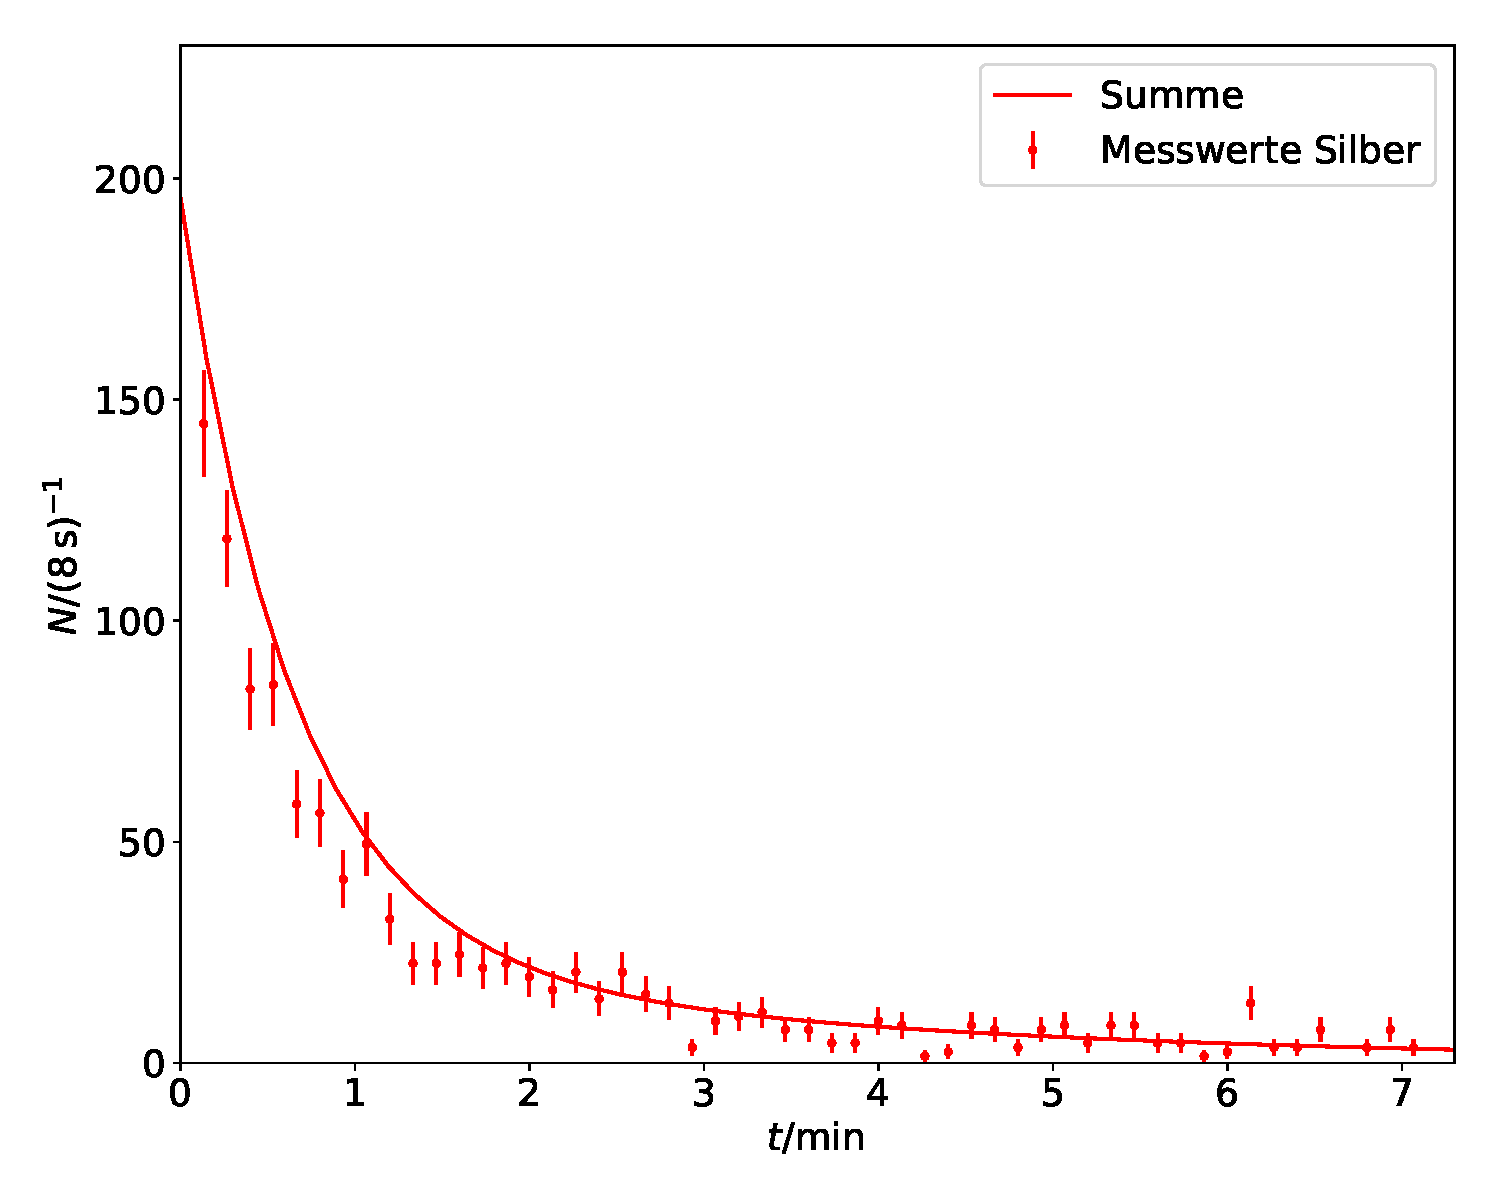
\includegraphics[width=\textwidth]{2Silber.pdf}
  \caption{Diagramm der vom Nulleffekt bereinigten Messwerte mit Summenkurve.}
  \label{fig:7}
\end{figure}
\section{Diskussion}
\begin{table}
  \centering
  \begin{tabular}{c c c c}
    \toprule
    Isotop & Quelle & $\mu$ & $T$\\
    \midrule
    $\ce{^{108}Ag}$ & \cite{Ag-108} & \SI[per-mode=reciprocal]{4.9e-3}{\per\second} & \SI{2.37}{\minute} \\
    $\ce{^{110}Ag}$ & \cite{Ag-110} & \SI[per-mode=reciprocal]{2.8e-2}{\per\second} & \SI{24.6}{\second} \\
    $\ce{^{116}In}$ & \cite{In-116} & \SI[per-mode=reciprocal]{2.1e-4}{\per\second} & \SI{54.29}{\minute} \\
    \bottomrule
  \end{tabular}
  \caption{Literaturwerte.}
  \label{tab:3}
\end{table}
In Tabelle \ref{tab:3} finden sich Literaturwerte für die einzellnen Isotope. Für
beide Silberisotope liegen die Theoriewerte sowohl für
Zerfallskonstante als auch für Halbwertszeit im Fehlerintervall der berechneten Werte.
Die Abweichung der nominellen Werte von den Literaturwerten ist bei der Messung des
kurzlebigeren $\ce{^{110}Ag}$ signifikant größer als bei $\ce{^{108}Ag}$. Dies ist darauf
zurückzuführen, dass auf dem Weg zwischen Anregungsbehälter und Messaufbau bereits eine
signifikante Menge an Zerfallsprozessen des kurzlebigeren Isotops stattgefunden hat,
sodass die Messwerte verfälscht werden. Dies ist beim langlebigeren Isotop ein
geringeres Problem. Die guten Ergebnisse für Silber spiegeln sich auch in der Summenkurve
wieder, die gut auf die Messwerte passt.\\
Für $\ce{^{116}In}$ gibt es keinen Wert, der im Bereich der Messtolleranz liegt.
Die relativen Fehler sind jedoch mit \SI{5.91}{\percent} für die Halbwertszeit
und \SI{4.76}{\percent} für die Zerfallskonstante gering. Mögliche Fehlerquelle
sind hier statistische Schwankungen. Widerholte Messungen
würde genauere Ergebnisse bringen.
\newpage
\nocite{*}
\printbibliography
